\chapter{Cost estimation}

\section{Function point}

\subsection{Brief introduction}
The Function Point estimation approach is based on the principle of extracting functions from a software, to classify them using a well defined set of classes and estimating their complexity.

This kind of estimation is extremely useful since it can be done at a very early stage of a project life-cycle, ideally after the implementation of the RASD.

This estimation is a single number called UFP that can be computed using a simple formula.

A high-level procedure that explains how to calculate this number is the following:

\begin{enumerate}
\item Classify each function of the software to one of these five possible classes called Function Types (explained in detail later):
\begin{itemize}
\item Internal logic files
\item External logic interfaces files
\item External Inputs
\item External outputs
\item External inquiries
\end{itemize}
\item For each function a complexity is defined, and it can be:
\begin{itemize}
\item Low
\item Average
\item High
\end{itemize}
The choice of the complexity is based on the analysis of the quantity of data processed by each function and takes into account also the type of interaction required between different components.
\item Calculate the UFP using the formula:
\[ \sum_{f\in F, c\in C} ((\sharp \text{ of function of type } f \text{ and complexity }c)*(\sharp \text{ weight for type } f \text{ and complexity }c)) \]
where F={ILF, ELF, EI, EO, EIQ} and C={Low, Average, High}. \\
Refer to this table to determine the proper weight for each type and complexity:
\begin{table}[!h]
\centering
\caption{UFP Complexity Weights}
\label{ufp-complex}
\begin{tabular}{cccc}
\hline
Function type             & Low & Average & High \\ \hline
Internal Logic files      & 7   & 10      & 15 \\
External Interfaces files & 5   & 7       & 10 \\
External Inputs           & 3   & 4       & 6  \\
External Ouputs           & 4   & 5       & 7  \\
External Inquiries        & 3   & 4       & 6  \\ \hline
\end{tabular}
\end{table}
\end{enumerate}

Further manipulation of the UFP can be done in order to use it in Cost Estimation Models such as COCOMO, but this will be explained later.

\clearpage
\subsection{Internal Logic Files}
The application manages a database which is used to store different kind of entities, each one of them has its own data structure.

These entities are: registered Client, system administrator, car, safe area, reservation/request, rent, transaction.

\begin{table}[!h]
\centering
\caption{ILF recap}
\label{itl-recap}
\begin{tabularx}{\linewidth}{XXc}
\hline
\textbf{ILF}                       & \textbf{Complexity} & \textbf{FP} \\ \hline
Registered client         & Low        & 7 \\
System administrator      & Low        & 7   \\
Car                       & Low        & 7  \\
Safe area                 & Average    & 10  \\
Reservation/Request       & High       & 15   \\
Rent                      & Average    & 10 \\
Transaction               & Average    & 10 \\ \hline
\textbf{Total:}           &            & \textbf{66}
\end{tabularx}
\end{table}

\subsection{External interface files}
The application of Power EnJoy must interact with some external services in order to fulfill its main goals.

The external services are about: driving License, maps, payment gateway, SMS gateway, push notification gateway, customer support.

\begin{table}[!h]
\centering
\caption{EIF recap}
\label{etl-recap}
\begin{tabularx}{\linewidth}{XXc}
\hline
\textbf{ELF}                       & \textbf{Complexity} & \textbf{FP} \\ \hline
Driving License           & Low        & 5 \\
Maps                      & High       & 10   \\
Payment gateway           & Average    & 7  \\
SMS gateway               & Low        & 5 \\
Push notification gateay  & Low        & 5 \\
Customer support          & Low        & 5 \\ \hline
\textbf{Total:}           &            & \textbf{37}
\end{tabularx}
\end{table}


\subsection{External Inputs }
The application has to handle external interactions due to the Registered Client’s actions or to the System Administrator’s actions.

These external interactions are: registration, login, logout, modify profile, make a reservation, choose a destination, terminate a rent, manage cars (System Administrator).

\begin{table}[!h]
\centering
\caption{EI recap}
\label{ei-recap}
\begin{tabularx}{\linewidth}{XXc}
\hline
\textbf{EI}                        & \textbf{Complexity} & \textbf{FP} \\ \hline
Registration              & Low        & 3  \\
Login                     & Low        & 3  \\
Logout                    & Low        & 3 \\
Modify profile            & Low        & 3  \\
Make a reservation        & High       & 6 \\
Chose a destination       & Average    & 4 \\
Terminate a rent          & High       & 6 \\
Cancel a reservation      & High       & 6 \\
Manage cars (SystemAdmin) & Average    & 4 \\ \hline
\textbf{Total:}           &            & \textbf{38}
\end{tabularx}
\end{table}

\subsection{External Outputs}
The application generates the following outputs, result of an internal computation on some data, to the Registered Client or to the System Administrator:

\begin{table}[!h]
\centering
\caption{EO recap}
\label{eo-recap}
\begin{tabularx}{\linewidth}{XXc}
\hline
\textbf{EO}                                      & \textbf{Complexity} & \textbf{FP}     \\ \hline
Best destination for getting a discount & High       & 7 \\
List of available cars                  & Low        & 4 \\
Notifications                           & Low        & 4 \\ \hline
\textbf{Total:}                         &            & \textbf{38}
\end{tabularx}
\end{table}

\subsection{External Inquiries}
The application generates the following outputs to the Registered Client or to the System Administrator:

\begin{table}[!h]
\centering
\caption{EInq recap}
\label{einq-recap}
\begin{tabularx}{\linewidth}{XXc}
\hline
\textbf{EInq}                                    & \textbf{Complexity} & \textbf{FP} \\ \hline
Show Registered Client profile          & Low        & 3 \\
Show System Administrator profile       & Low        & 3 \\
Show history of past rents              & Low        & 3 \\
Show current cost, charge and maps through the OnBoard application & Average & 4 \\ \hline
\textbf{Total:}                         &            & \textbf{14}
\end{tabularx}
\end{table}

\subsection{Recap}
The following table summarizes the amount of FP for each type and the overall sum that corresponds to the final UFP value.

\begin{table}[!h]
\centering
\caption{Function point recap}
\label{einq-recap}
\begin{tabularx}{\linewidth}{Xc}
\hline
\textbf{Function type}            & \textbf{Value}      \\ \hline
Internal logic files       & 66 \\
External interfaces files  & 37 \\
External inputs            & 38 \\
External outputs           & 15 \\
External inquiries         & 13 \\ \hline
\textbf{Total:}            & \textbf{169}
\end{tabularx}
\end{table}

\[ \sum_{f\in F, c\in C} ((\sharp \text{ of function of type } f \text{ and complexity }c)*(\sharp \text{ weight for type } f \text{ and complexity }c)) = 169 \]

\clearpage
\section{COCOMO}

\subsection{Brief introduction}
The aim of using COCOMO is to obtain an estimation of the effort needed to develop the software in analysis.
The effort is defined by the following formula:

\[ \text{Effort} = A \cdot SLOC^{E} \cdot\prod_{i=1}^nEM_{i} \]

The elements considered to define the values for the estimation are based not only on technical drivers like SLOC or complexity of the software, but also on intrinsic variables like workforce and business processes.

\subsection{Lines of Codes}
Code size is expressed in thousands of source lines of code (KSLOC).
In order to estimate this parameter we consider the value of the UFP and we convert it using the standard value indicated in COCOMO II for JavaScript.
So we obtain the following values:
\begin{itemize}
\item Lower bound: \( SLOC = 169 \cdot 31 = 5239 = 5,239 KSLOC \)
\item Average bound: \( SLOC = 169 \cdot 31 = 7943 = 7,943 KSLOC \)
\item Upper bound: \( SLOC = 169 \cdot 63 = 10647 = 10,647 KSLOC \)
\end{itemize}

From now on we consider for our analysis the average value of 7,943 KSLOC.

\subsection{Scale Drivers}
Scale drivers are factors used to calculate the exponent E of the Effort equation defined above.
E can be computed using this equation:
\[ E = B + 0.01 \cdot \sum_{j=1}^fSF_j \]
We can distinguish three different cases:
\begin{itemize}
\item If \( E < 1.0 \), the project exhibits economies of scale.
\item If \( E = 1.0 \), the economies and diseconomies of scale are in balance.
\item If \( E > 1.0 \), the project exhibits diseconomies of scale.
\end{itemize}

In this section five factors are considered to evaluate E:
\begin{itemize}
\item Precedentedness: it measures the experience related to the kind of project and development, that derives from similarity of projects previously developed.
We set this parameter to low.
\item Development flexibility: it expresses the capacity of development team to adapt itself to changes during the development process.
In particular it measures how much the software needs to be accurate with the respect to the initial requirements and to the external interfaces.
We set this scale driver to nominal.
\item Risk resolution: it expresses the amount of effort and budget to be invested in order to predict and manage risks that can occur during the life cycle of the software.
We set this parameter to nominal.
\item Team cohesion: it represents the capabilities of all the actors involved in the development process to communicate and interact with the aim of reach the result expected.
We set this scale driver to very high.
\item Process maturity: it’s a parameter indicating the ability to manage development processes, like defect management, quality assurance, change management, etc.
In particular it gives a measure of how much sophisticated the development of the project is, basing the analysis on some general criteria.
We set this scale driver to high.
\end{itemize}

\begin{minipage}{\textwidth}
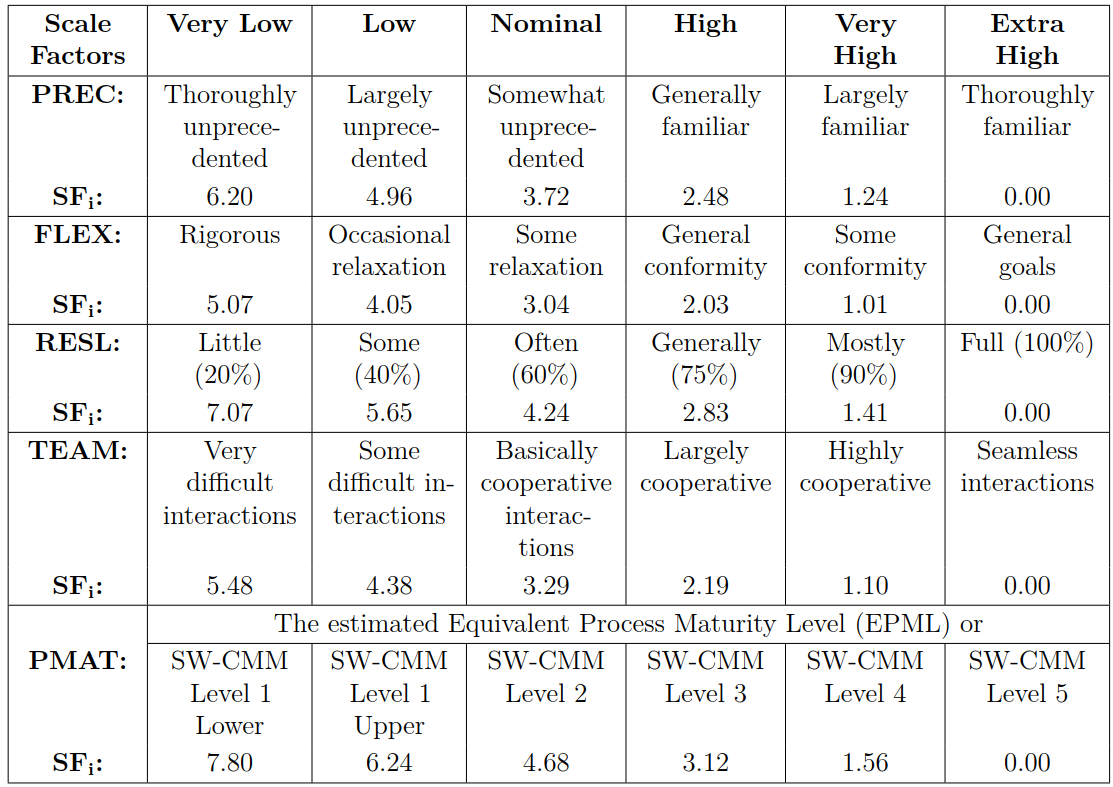
\includegraphics[width=\textwidth, keepaspectratio]{../images/scale_factors_generic.png}
\captionof{figure}{Scale factor values, \( SF_i \), for COCOMO II Models}
\end{minipage}

In the following table we recap the values we have chosen for the Scale Factors.

\begin{table}[!h]
\centering
\caption{Scale factors recap}
\label{scalefact-recap}
\begin{tabularx}{\linewidth}{XXc}
\hline
\textbf{Scale Driver}                & \textbf{Selected Factor} & \textbf{Value} \\ \hline
Precedentedness                      & Low                      & 4.96 \\
Development flexibility              & Nominal                  & 3.04 \\
Risk resolution              & Nominal                  & 4.24 \\
Team cohesion              & Very High                  & 3.12 \\
Process maturity              & High                  & 3.04 \\ \hline
\textbf{Total:}                      &                          & \textbf{17.55} \\
\end{tabularx}
\end{table}

\subsection{Cost Drivers}
Cost Drivers are model factors which aim is to take into account the main characteristics of the software development, characteristics that influence the cost.
The main Cost Drivers and their standard respective multipliers that we consider are:
\begin{itemize}
\item \textbf{Required Software Reliability:} this measures the extent to which the software must perform its functions over a period of time. We set this parameter to nominal.

\begin{minipage}{\textwidth}
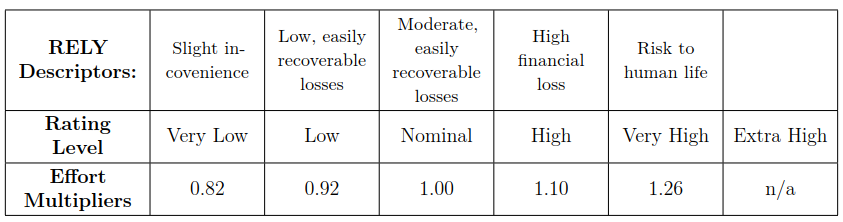
\includegraphics[width=\linewidth-1cm, keepaspectratio]{../images/cost_driver/RELY.png}
\captionof{figure}{RELY cost driver}
\end{minipage}
\item \textbf{Database size:} this measure is related to the dimension of the database. The reason to do it is to consider the effort required to generate the test data that will be used to exercise the program. In our case its value is nominal.

\begin{minipage}{\textwidth}
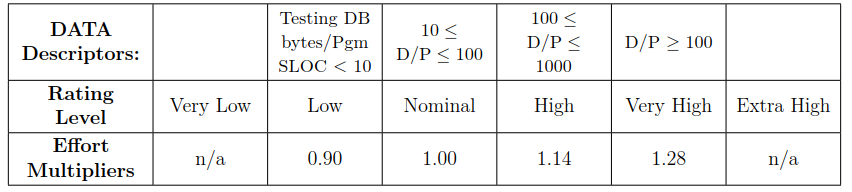
\includegraphics[width=\linewidth-1cm, keepaspectratio]{../images/cost_driver/data.png}
\captionof{figure}{DATA cost driver}
\end{minipage}
\item \textbf{Product complexity:} the complexity is derived consider five different areas: control operations, computational operations, device-dependent operations, data management operations, and user interface management operations. We set this parameter to high.

\begin{minipage}{\textwidth}
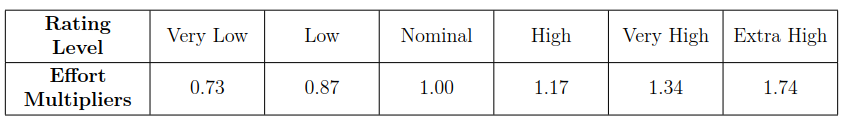
\includegraphics[width=\linewidth-1cm, keepaspectratio]{../images/cost_driver/cplx.png}
\captionof{figure}{CPLX cost driver}
\end{minipage}
\item \textbf{Required reusability:} this cost driver estimates the effort needed to create new components that have to reuse the current project. We set set this parameter to high.

\begin{minipage}{\textwidth}
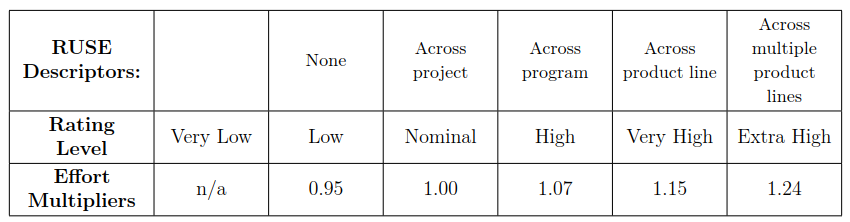
\includegraphics[width=\linewidth-1cm, keepaspectratio]{../images/cost_driver/ruse.png}
\captionof{figure}{RUSE cost driver}
\end{minipage}
\item \textbf{Documentation match to life-cycle needs:} it measures the suitability of the documentation of the project with its real life usage characteristics. We set this parameter to nominal.

\begin{minipage}{\textwidth}
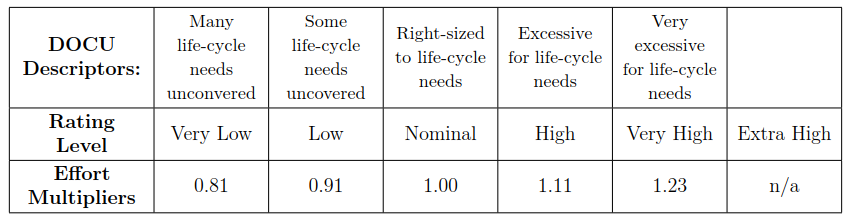
\includegraphics[width=\linewidth-1cm, keepaspectratio]{../images/cost_driver/docu.png}
\captionof{figure}{DOCU cost driver}
\end{minipage}
\item \textbf{Execution time constraint:} this measure states an execution time constraint and is expressed in terms of the percentage of available execution time expected to be used by the system or by a subsystem. We set this parameter to nominal.

\begin{minipage}{\textwidth}
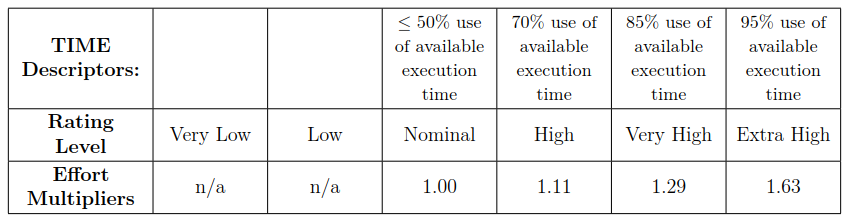
\includegraphics[width=\linewidth-1cm, keepaspectratio]{../images/cost_driver/time.png}
\captionof{figure}{TIME cost driver}
\end{minipage}
\item \textbf{Storage constraint:} this parameter describes the expected amount of storage usage with respect to the availability of the hardware. We set this parameter to nominal.

\begin{minipage}{\textwidth}
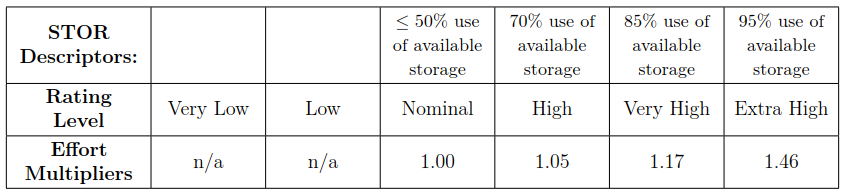
\includegraphics[width=\linewidth-1cm, keepaspectratio]{../images/cost_driver/stor.png}
\captionof{figure}{STOR cost driver}
\end{minipage}
\item \textbf{Platform Volatility:} with the term platform we indicates both software and hardware that the software has to call in order to pursue its tasks. This factor measures the probability of our platform to be changed. We set this parameter to high.

\begin{minipage}{\textwidth}
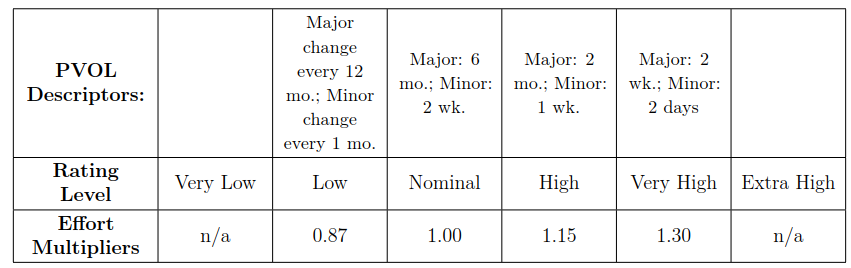
\includegraphics[width=\linewidth-1cm, keepaspectratio]{../images/cost_driver/pvol.png}
\captionof{figure}{PVOL cost driver}
\end{minipage}
\item \textbf{Analyst Capability:} this measures analysts’ abilities, capacity of communication and efficiency. We set this parameter to very high.

\begin{minipage}{\textwidth}
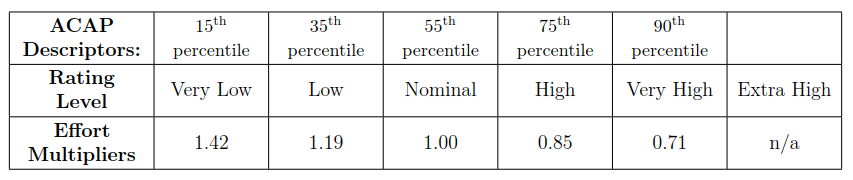
\includegraphics[width=\linewidth-1cm, keepaspectratio]{../images/cost_driver/acap.png}
\captionof{figure}{ACAP cost driver}
\end{minipage}
\item \textbf{Programmer Capability:} this factor measures the capability of programmers to work as individuals and in a team. We set this parameter to very high.

\begin{minipage}{\textwidth}
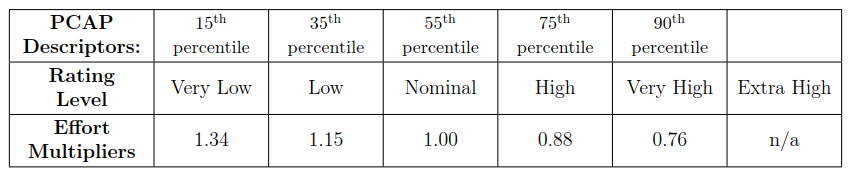
\includegraphics[width=\linewidth-1cm, keepaspectratio]{../images/cost_driver/pcap.png}
\captionof{figure}{PCAP cost driver}
\end{minipage}
\item \textbf{Application Experience:} this cost driver depends on the level of experience that the project team have to develop the software system or subsystem. We set this parameter to nominal.

\begin{minipage}{\textwidth}
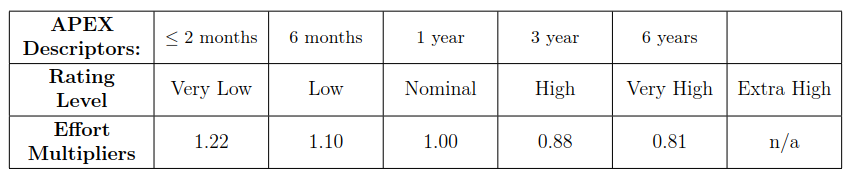
\includegraphics[width=\linewidth-1cm, keepaspectratio]{../images/cost_driver/apex.png}
\captionof{figure}{APEX cost driver}
\end{minipage}
\item \textbf{Platform Experience:} this factor measures the experience on the usage of the platform. We set this parameter to nominal.

\begin{minipage}{\textwidth}
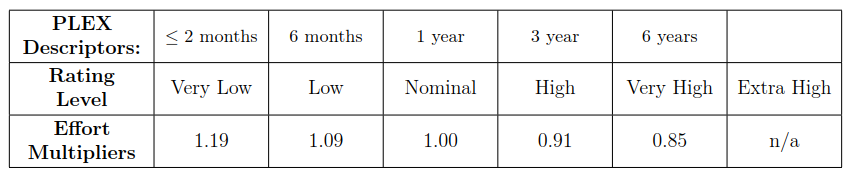
\includegraphics[width=\linewidth-1cm, keepaspectratio]{../images/cost_driver/plex.png}
\captionof{figure}{PLEX cost driver}
\end{minipage}
\item \textbf{Language and Tool Experience:} this is a measure of the level of programming language and software tool experience of the project team developing the software system or subsystem. We consider this value as nominal.

\begin{minipage}{\textwidth}
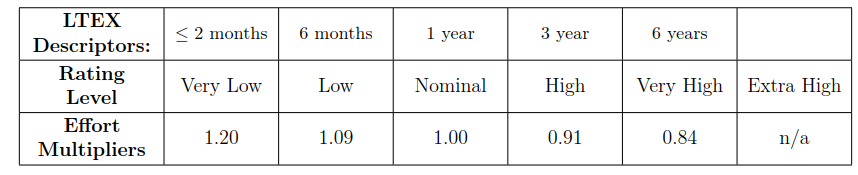
\includegraphics[width=\linewidth-1cm, keepaspectratio]{../images/cost_driver/ltex.png}
\captionof{figure}{LTEX cost driver}
\end{minipage}
\item \textbf{Personnel continuity:} it expresses a measure of the project’s annual personnel turnover. We consider this value as very low.

\begin{minipage}{\textwidth}
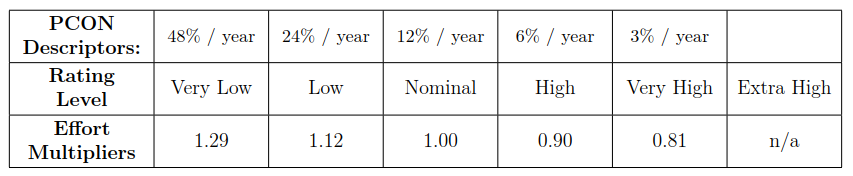
\includegraphics[width=\linewidth-1cm, keepaspectratio]{../images/cost_driver/pcon.png}
\captionof{figure}{PCON cost driver}
\end{minipage}
\item \textbf{Usage of Software Tools:} this parameter is set considering the effort needed to develop and  integrate all the tools that the software requires. The value of this parameter is high.

\begin{minipage}{\textwidth}
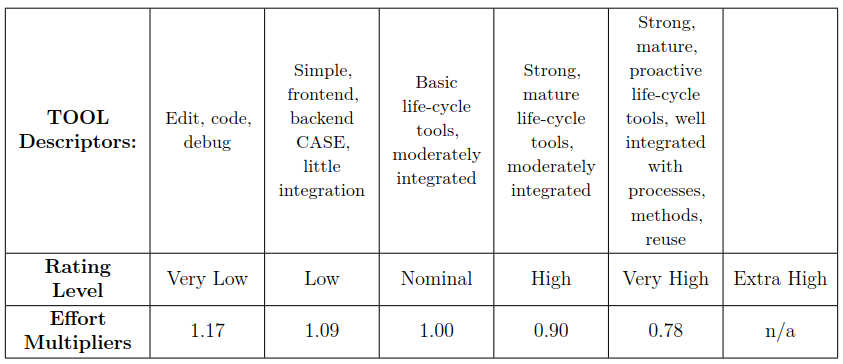
\includegraphics[width=\linewidth-1cm, keepaspectratio]{../images/cost_driver/tool.png}
\captionof{figure}{TOOL cost driver}
\end{minipage}
\item \textbf{Multi-site development:} this cost driver has been chosen considering two factors: site collocation and communication support. We set this parameter to high.

\begin{minipage}{\textwidth}
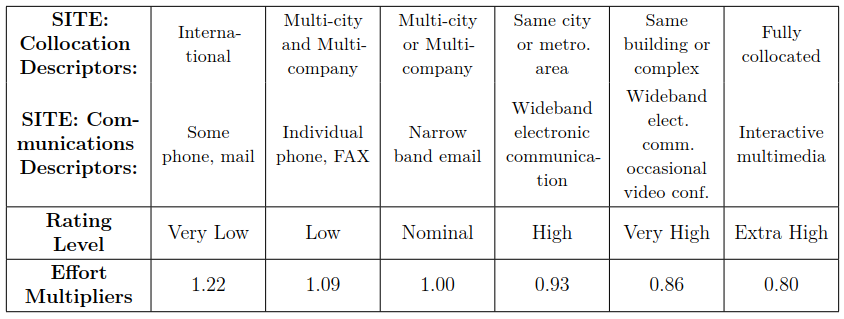
\includegraphics[width=\linewidth-1cm, keepaspectratio]{../images/cost_driver/site.png}
\captionof{figure}{SITE cost driver}
\end{minipage}
\item \textbf{Required development schedule:} this cost driver measures the schedule constraints imposed on the project team developing the software. The ratings are defined in percentage of schedule stretch-outs or accelerations with respect to a nominal schedule for a project requiring a given amount of effort. We set this parameter to nominal.

\begin{minipage}{\textwidth}
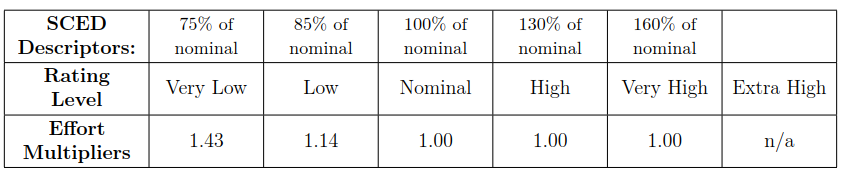
\includegraphics[width=\linewidth-1cm, keepaspectratio]{../images/cost_driver/sced.png}
\captionof{figure}{SCED cost driver}
\end{minipage}
\end{itemize}

\clearpage
\subsection{Cost driver recap}
In the following table we recap the values we have chosen for the Cost Drivers.

\begin{table}[!h]
\centering
\caption{Cost factors recap}
\label{costdriver-recap}
\begin{tabularx}{\linewidth}{XXc}
\hline
\textbf{Cost Driver}                & \textbf{Selected Factor} & \textbf{Value} \\ \hline
Required Software Reliability       & Nominal                  & 1.00 \\
Database Size                       & Nominal                  & 1.00 \\
Product Complexity                  & High                     & 1.17 \\
Required Reusability                & High                     & 1.07 \\
Documentation match to life-cycle needs & Nominal              & 1.00 \\
Execution Time Constraint           & Nominal                  & 1.00 \\
Main Storage Constraint             & Nominal                  & 1.00 \\
Platform Volatility                 & High                     & 1.15 \\
Analyst Capability                  & High                     & 0.85 \\
Programmer Capability               & High                     & 0.88 \\
Application Experience              & Nominal                  & 1.00 \\
Platform Experience                 & Nominal                  & 1.00 \\
Language and Tool Experience        & Nominal                  & 1.00 \\
Personnel Continuity                & Very Low                 & 1.29 \\
Usage of Software Tools             & High                     & 0.90 \\
Multi-site Development              & High                     & 0.93 \\
Required Development Schedule       & Nominal                  & 1.00 \\ \hline
\textbf{Product:}                   &                          & \textbf{1.16}
\end{tabularx}
\end{table}

\[ \prod_{i=1}^nEM_{i} = 1.16 \]

\subsection{Effort computation}
Using the values obtained in the previous section we can estimate duration and effort.
Given the standard value of COCOMO II A = 2.94, B = 0.91, C=3.67 and D= 0.28, we have:

\[ E = B + 0.01 \cdot \sum_{j=1}^{5}SF_j = 0.91 + 0.01 \cdot 17.55 = 1.0855  \]

\[ EAF = \prod_{i=1}^{n} EM_{i} = 1.16 \]

\[ \text{Effort} = A \cdot EAF \cdot KSOLC^{E} = 2.94 \cdot 1.16 \cdot 7,943 ^{1.0855} = 32.33 \text{ person/month} \]

\[ ( D + 0.2 \cdot (E -B)) =  (0.28 + 0.2 \cdot(1.0855 - 0.91)) = 0.3151 \]

\[ \text{Duration} = [C \cdot (PM)^{D+0.2 \cdot(E-B)}] = [3.67 \cdot (32.33)^{0.3151}] = 10.97 = 11\text{ months} \]

\[ N = \text{ number of people needed } = \text{ Effort/Duration } = 32.33/11 = 2.93 = 3 \text{ people} \]